% Figure 1 (draft): the membership game and the three mechanism-aware attacks.
% Standalone; build with  tectonic -X compile overview.tex  (gives overview.pdf,
% 18 cm wide, included at \textwidth, so the type sizes below are final:
% 8 pt titles, 7 pt text, 6 pt annotations).
% Colours match scripts/paper_figures.py: one colour per attack family.
\documentclass[tikz,border=1pt]{standalone}
\usepackage{fontspec}
\setmainfont{texgyreheros}[Extension=.otf,UprightFont=*-regular,BoldFont=*-bold,ItalicFont=*-italic,BoldItalicFont=*-bolditalic]
\setsansfont{texgyreheros}[Extension=.otf,UprightFont=*-regular,BoldFont=*-bold,ItalicFont=*-italic,BoldItalicFont=*-bolditalic]
\usepackage[italic]{mathastext}
\usetikzlibrary{arrows.meta,calc,decorations.pathreplacing}

\definecolor{ink}{HTML}{0B0B0B}
\definecolor{ink2}{HTML}{52514E}
\definecolor{muted}{HTML}{898781}
\definecolor{hair}{HTML}{C3C2B7}
\definecolor{grid}{HTML}{E1E0D9}
\definecolor{mahala}{HTML}{2A78D6}
\definecolor{melo}{HTML}{EB6834}
\definecolor{mama}{HTML}{1BAF7A}
\definecolor{expr}{HTML}{3D4A5C}

\newcommand{\ttl}{\fontsize{8}{9.6}\selectfont\bfseries}
\newcommand{\txt}{\fontsize{7}{8.4}\selectfont}
\newcommand{\ann}{\fontsize{6}{7.2}\selectfont}

\tikzset{
  >={Stealth[length=4pt,width=3.4pt]},
  flow/.style={->,draw=ink2,line width=0.7pt},
  ann/.style={font=\ann,text=ink2,align=center,inner sep=1.5pt},
  txt/.style={font=\txt,text=ink,align=left,inner sep=1.5pt},
  box/.style={draw=hair,rounded corners=2pt,line width=0.6pt,fill=white,
              font=\txt,text=ink,align=center,inner sep=2pt,minimum height=0.68cm},
  synth/.style={box,fill=melo!13,draw=melo!65},
  member/.style={circle,fill=ink,inner sep=0pt,minimum size=3.8pt},
  nonmember/.style={circle,draw=ink,fill=white,line width=0.7pt,inner sep=0pt,minimum size=3.8pt},
}

% \exprmatrix{x}{top y}{rows}{cols}{seed}{gap after row}: a block of expression values
\newcommand{\exprmatrix}[6]{%
  \pgfmathsetseed{#5}%
  \foreach \i in {1,...,#3}{%
    \foreach \j in {1,...,#4}{%
      \pgfmathsetmacro{\v}{int(10+68*rnd)}%
      \pgfmathsetmacro{\yy}{#2-0.15*\i-(\i>#6 ? 0.1 : 0)}%
      \fill[expr!\v!white] ({#1+0.15*(\j-1)},\yy) rectangle ++(0.135,0.135);
    }}}

% \card{x}{colour}{name}{what it reads}{against}
\newcommand{\card}[5]{%
  \draw[draw=#2!60,line width=0.7pt,rounded corners=3pt,fill=white] (#1,0) rectangle ++(5.85,5.0);
  \fill[#2,rounded corners=3pt] (#1,4.48) rectangle ++(5.85,0.52);
  \fill[#2] (#1,4.48) rectangle ++(5.85,0.2);
  \node[anchor=west,font=\ttl,text=white] at (#1+0.1,4.74) {#3};
  \node[anchor=east,font=\txt,text=white] at (#1+5.75,4.74) {#4};
  \node[anchor=west,font=\txt,text=ink2] at (#1+0.1,4.17) {against #5};
}

\begin{document}
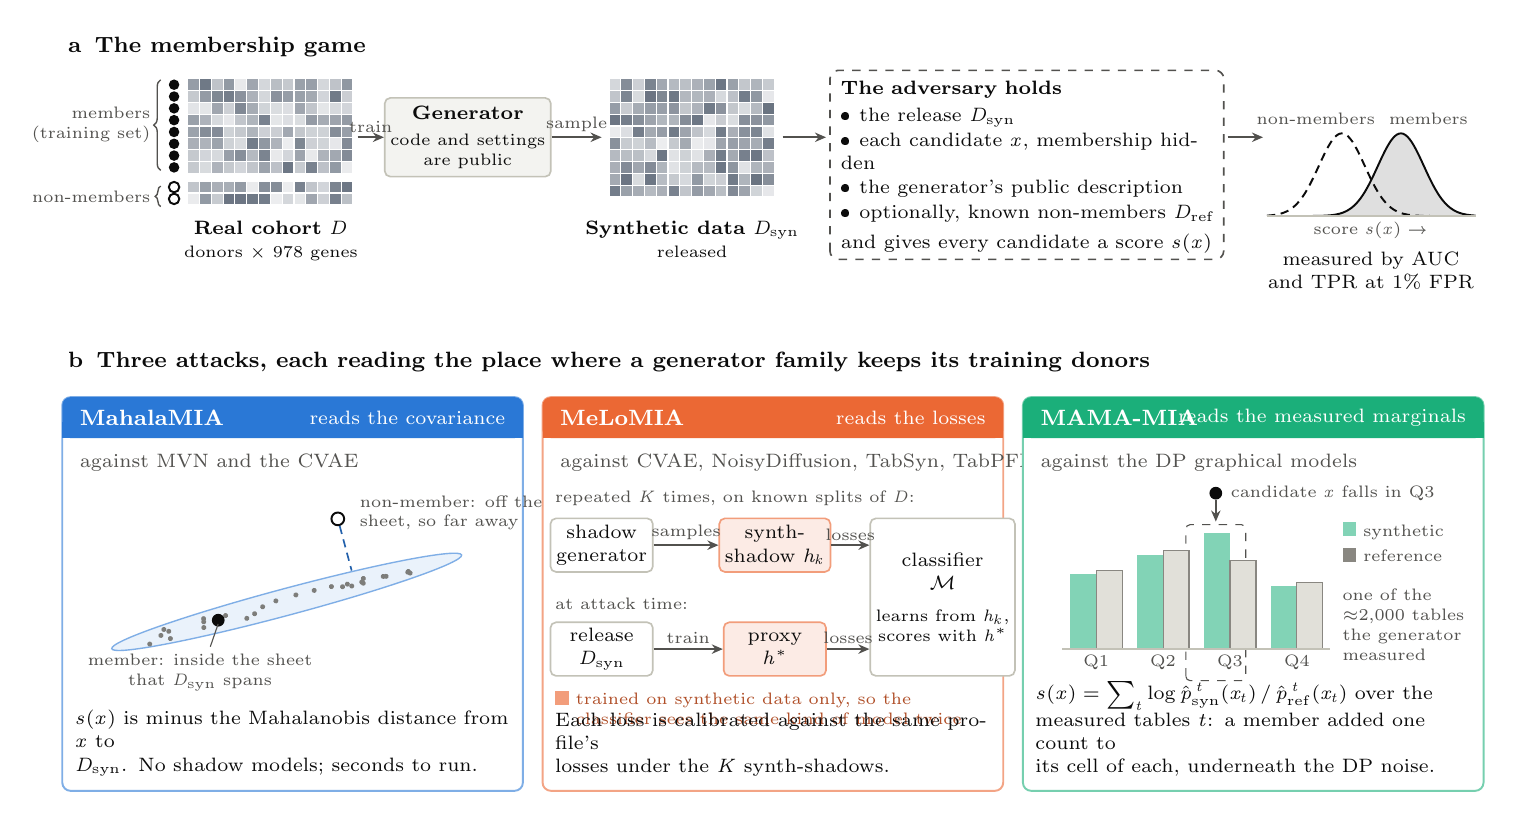
\begin{tikzpicture}

% ============================ (a) the membership game ============================
\node[anchor=west,font=\ttl,text=ink] at (-0.05,9.45) {a\enspace The membership game};

% real cohort: rows are donors, columns genes; 8 members, then 2 held-out donors
\exprmatrix{1.6}{9.05}{10}{14}{11}{8}
\foreach \i in {1,...,8} \node[member] at (1.42,{9.05-0.15*\i+0.0675}) {};
\foreach \i in {9,10} \node[nonmember] at (1.42,{9.05-0.15*\i+0.0675-0.1}) {};
\draw[decorate,decoration={brace,amplitude=2.5pt,mirror},draw=ink2,line width=0.5pt]
  (1.25,9.03) -- node[left=2pt,ann,align=right] {members\\(training set)} (1.25,7.88);
\draw[decorate,decoration={brace,amplitude=2pt,mirror},draw=ink2,line width=0.5pt]
  (1.25,7.68) -- node[left=2pt,ann,align=right] {non-members} (1.25,7.42);
\node[txt,anchor=north,align=center] at (2.65,7.3) {\textbf{Real cohort} $D$\\{\ann donors $\times$ 978 genes}};

% generator
\node[box,minimum width=1.75cm,minimum height=1.0cm,fill=grid!40] (gen) at (5.15,8.3)
  {\textbf{Generator}\\[1pt]{\ann code and settings}\\[-1pt]{\ann are public}};
\draw[flow] (3.75,8.3) -- node[above,ann] {train} (gen.west);

% synthetic release
\exprmatrix{6.95}{9.05}{10}{14}{29}{10}
\draw[flow] (gen.east) -- node[above,ann] {sample} (6.85,8.3);
\node[txt,anchor=north,align=center] at (8.0,7.3) {\textbf{Synthetic data} $D_{\mathrm{syn}}$\\{\ann released}};

% adversary
\draw[draw=ink2,dashed,line width=0.6pt,rounded corners=3pt] (9.75,6.75) rectangle (14.75,9.15);
\node[anchor=north west,txt,text width=4.8cm] at (9.83,9.08) {%
  \textbf{The adversary holds}\\[1.5pt]
  \textbullet\ the release $D_{\mathrm{syn}}$\\[0.5pt]
  \textbullet\ each candidate $x$, membership hidden\\[0.5pt]
  \textbullet\ the generator's public description\\[0.5pt]
  \textbullet\ optionally, known non-members $D_{\mathrm{ref}}$\\[2.5pt]
  and gives every candidate a score $s(x)$};
\draw[flow] (9.15,8.3) -- (9.7,8.3);

% outcome: score distributions of members and non-members
\begin{scope}[shift={(15.3,7.3)}]
  \fill[ink!13] plot[domain=0:2.65,samples=50,smooth] (\x,{1.05*exp(-((\x-1.7)^2)/0.17)}) -- (2.65,0) -- (0,0) -- cycle;
  \draw[ink,line width=0.7pt] plot[domain=0:2.65,samples=50,smooth] (\x,{1.05*exp(-((\x-1.7)^2)/0.17)});
  \draw[ink,line width=0.7pt,densely dashed] plot[domain=0:2.65,samples=50,smooth] (\x,{1.05*exp(-((\x-0.95)^2)/0.17)});
  \draw[hair,line width=0.5pt] (0,0) -- (2.65,0);
  \node[ann,anchor=south] at (0.62,1.1) {non-members};
  \node[ann,anchor=south] at (2.05,1.1) {members};
  \node[ann,anchor=north] at (1.32,-0.02) {score $s(x)$ \textrightarrow};
  \node[txt,anchor=north,align=center] at (1.32,-0.4) {measured by AUC\\and TPR at 1\% FPR};
\end{scope}
\draw[flow] (14.8,8.3) -- (15.25,8.3);

% ======================= (b) where each attack reads ===========================
\node[anchor=west,font=\ttl,text=ink] at (-0.05,5.45)
  {b\enspace Three attacks, each reading the place where a generator family keeps its training donors};

% ---------------- MahalaMIA ----------------
\card{0}{mahala}{MahalaMIA}{reads the covariance}{MVN and the CVAE}
\begin{scope}[shift={(2.85,2.4)},rotate=15]
  \fill[mahala!10] (0,0) ellipse (2.3 and 0.17);
  \draw[mahala!60,line width=0.5pt] (0,0) ellipse (2.3 and 0.17);
  \pgfmathsetseed{5}
  \foreach \k in {1,...,28}{
    \pgfmathsetmacro{\u}{2.05*rand}\pgfmathsetmacro{\w}{0.075*rand}
    \fill[ink2!75] (\u,\w) circle (0.032);}
  \node[member,minimum size=4.6pt] at (-0.9,0.0) {};
  \node[nonmember,minimum size=4.6pt] (n) at (0.9,0.85) {};
  \draw[mahala!80!black,densely dashed,line width=0.6pt] (n) -- (0.9,0.17);
\end{scope}
\node[ann,anchor=west,align=left] at (3.72,3.53) {non-member: off the\\sheet, so far away};
\node[ann,anchor=north,align=center] at (1.75,1.8) {member: inside the sheet\\that $D_{\mathrm{syn}}$ spans};
\draw[ink2,line width=0.4pt] (1.98,2.12) -- (1.88,1.83);
\node[txt,anchor=south west,text width=5.6cm] at (0.1,0.12) {%
  $s(x)$ is minus the Mahalanobis distance from $x$ to\\
  $D_{\mathrm{syn}}$. No shadow models; seconds to run.};

% ---------------- MeLoMIA ----------------
\card{6.1}{melo}{MeLoMIA}{reads the losses}{CVAE, NoisyDiffusion, TabSyn, TabPFN}
\begin{scope}[shift={(6.1,0)}]
  \node[ann,anchor=west] at (0.1,3.72) {repeated $K$ times, on known splits of $D$:};
  \node[box,minimum width=1.3cm] (bs) at (0.75,3.12) {shadow\\generator};
  \node[synth,minimum width=1.3cm] (ss) at (2.95,3.12) {synth-\\shadow $h_k$};
  \draw[flow] (bs) -- node[above,ann] {samples} (ss);
  \node[ann,anchor=west] at (0.1,2.38) {at attack time:};
  \node[box,minimum width=1.3cm] (rel) at (0.75,1.8) {release\\$D_{\mathrm{syn}}$};
  \node[synth,minimum width=1.3cm] (px) at (2.95,1.8) {proxy\\$h^{\ast}$};
  \draw[flow] (rel) -- node[above,ann] {train} (px);
  \node[box,minimum width=1.25cm,minimum height=2.0cm] (clf) at (5.08,2.46)
    {classifier\\$\mathcal{M}$\\[3pt]{\ann learns from $h_k$,}\\[-1pt]{\ann scores with $h^{\ast}$}};
  \draw[flow] (ss.east) -- node[above,ann] {losses} (clf.west|-ss.east);
  \draw[flow] (px.east) -- node[above,ann] {losses} (clf.west|-px.east);
  \node[ann,anchor=north west,text=melo!75!black,align=left] at (0.1,1.33)
    {\textcolor{melo!65}{\rule{5pt}{5pt}}\ trained on synthetic data only, so the\\\phantom{\rule{5pt}{5pt}}\ classifier sees the same kind of model twice};
  \node[txt,anchor=south west,text width=5.6cm] at (0.1,0.12) {%
    Each loss is calibrated against the same profile's\\losses under the $K$ synth-shadows.};
\end{scope}

% ---------------- MAMA-MIA ----------------
\card{12.2}{mama}{MAMA-MIA}{reads the measured marginals}{the DP graphical models}
\begin{scope}[shift={(12.2,0)}]
  % one measured table: a gene cut at its quartiles; synthetic vs reference counts
  \draw[dashed,draw=ink2,line width=0.4pt,rounded corners=1.5pt] (2.07,1.4) rectangle (2.83,3.38);
  \foreach \b/\s/\r in {1/0.95/1.0, 2/1.2/1.25, 3/1.48/1.12, 4/0.8/0.85}{
    \fill[mama!55] ({0.6+0.85*(\b-1)},1.8) rectangle ++(0.33,\s);
    \fill[grid] ({0.93+0.85*(\b-1)},1.8) rectangle ++(0.33,\r);
    \draw[muted,line width=0.4pt] ({0.93+0.85*(\b-1)},1.8) rectangle ++(0.33,\r);
  }
  \draw[hair,line width=0.5pt] (0.5,1.8) -- (3.9,1.8);
  \foreach \b/\q in {1/Q1,2/Q2,3/Q3,4/Q4} \node[ann,anchor=north] at ({0.93+0.85*(\b-1)},1.78) {\q};
  \node[member,minimum size=4.6pt] (cx) at (2.45,3.78) {};
  \node[ann,anchor=west] at (2.58,3.78) {candidate $x$ falls in Q3};
  \draw[->,ink2,line width=0.5pt] (cx) -- (2.45,3.42);
  \node[ann,anchor=west,align=left] at (4.0,3.3) {\textcolor{mama!55}{\rule{5pt}{5pt}}\ synthetic};
  \node[ann,anchor=west,align=left] at (4.0,3.0) {\textcolor{muted}{\rule{5pt}{5pt}}\ reference};
  \node[ann,anchor=north west,align=left] at (4.0,2.62) {one of the\\$\approx$2,000 tables\\the generator\\measured};
  \node[txt,anchor=south west,text width=5.6cm] at (0.1,0.12) {%
    $s(x)=\sum_{t}\log\hat p^{\,t}_{\mathrm{syn}}(x_t)\,/\,\hat p^{\,t}_{\mathrm{ref}}(x_t)$ over the\\measured tables $t$: a member added one count to\\its cell of each, underneath the DP noise.};
\end{scope}

\end{tikzpicture}
\end{document}
